% !TEX root = trkjet.tex

The \Dptr\ distributions are studied as a function of \ptjet\ for \pp\ data and \PbPb\ collisions with different centralities. Ratios and differences between \Dptr\ distributions in \pbpb\ and \pp\ collisions are evaluated to explore the interplay between the hot and dense matter and the parton shower.

The \Dptr\ distributions evaluated in \pp\ and \pbpb\ collisions for $126 < \ptjet < 158$ GeV are shown in Figure~\ref{fig:dptr}. The distributions exhibit a difference in shape between \PbPb\ and the \pp\ reference, with the \pbpb\ distributions being broader at low \pt\ (\pt < 4 GeV) and narrower at high \pt\ (\pt > 4 GeV) in \mbox{0--10\%} central collisions. This modification is centrality dependent and is smaller for peripheral \pbpb\ collisions.

\begin{figure}[h]
\centerline{
            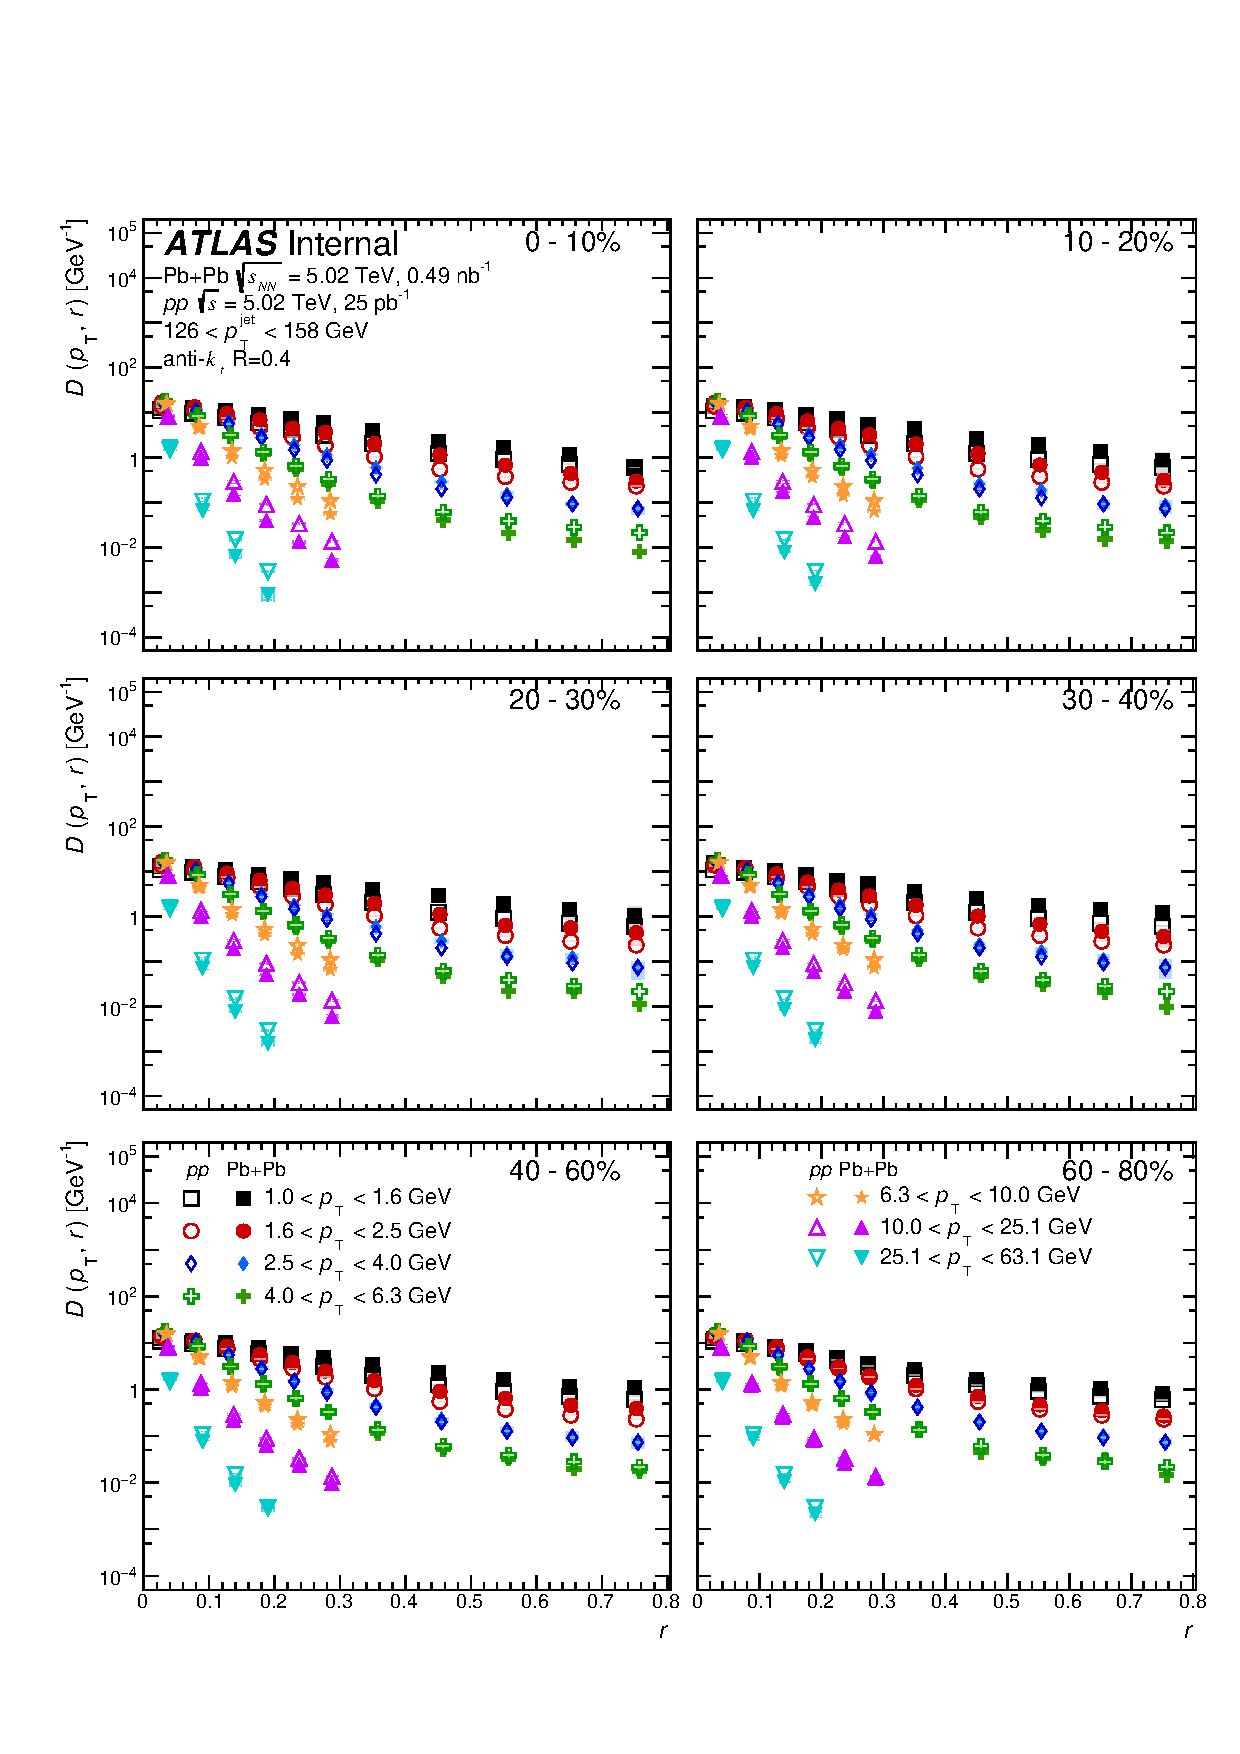
\includegraphics[width=1\textwidth]{figures/results/DpT_dR_jet7.pdf} 
      }
\caption{The \Dptr\ distributions in \pp\ (open symbols) and \pbpb\ (closed symbols) as a function of angular distance $r$ for \ptjet\ of 126 to 158~\GeV. The colors represent different track \pt\ ranges, and each panel is a different centrality selection. The vertical bars on the data points indicate statistical uncertainties while the shaded boxes indicate systematic uncertainties. The widths of the boxes are not indicative of the bin size and the points are shifted horizontally for better visibility.}
\label{fig:dptr}
\end{figure}


Ratios of the \Dptr\ distributions in \pbpb\ to those measured in \pp\ for $126 < \ptjet < 158$ GeV and $200 < \ptjet < 251$ GeV jets and are presented in Figure~\ref{fig:rdptr}. They are shown as a function of $r$ for different \pt\ and centrality selections. In 0--10\% central collisions,
\RDptr\ is above unity for $\rvar < 0.7$ for charged-particles with \pT less than 4~\GeV\ in both jet selections. 
For these particles, 
the enhancement of the charged particle spectra grows with increasing \rvar\ up to \mbox{$\rvar  = 0.3$}. It is approximately constant over \mbox{0.3 -- 0.6} and decreases for \mbox{$\rvar > 0.6$}.  For charged particles with $\pt > 4.0$ \GeV, \RDptr\ shows a depletion outside the jet core for $r > 0.05$. The magnitude of this depletion increases with increasing \rvar\ up to $r = 0.3$ and is approximately constant thereafter.
 The observed behavior inside the jet ($r < 0.4$) agrees with the measurement of the inclusive jet fragmentation functions~\cite{Aaboud:2017eww, PhysRevC.98.024908}, where yields of fragments with $\pt < 4$ GeV are observed to be enhanced and yields of charged particles with intermediate \pT\ are suppressed in \PbPb\ collisions compared to those in \pp\ for collisions. 
For peripheral collisions, \RDptr\ has no significant \rvar\ dependence and the distributions do not significantly deviate from unity. 

\begin{figure}[h]
\centerline{
         \begin{tabular}{cc}
            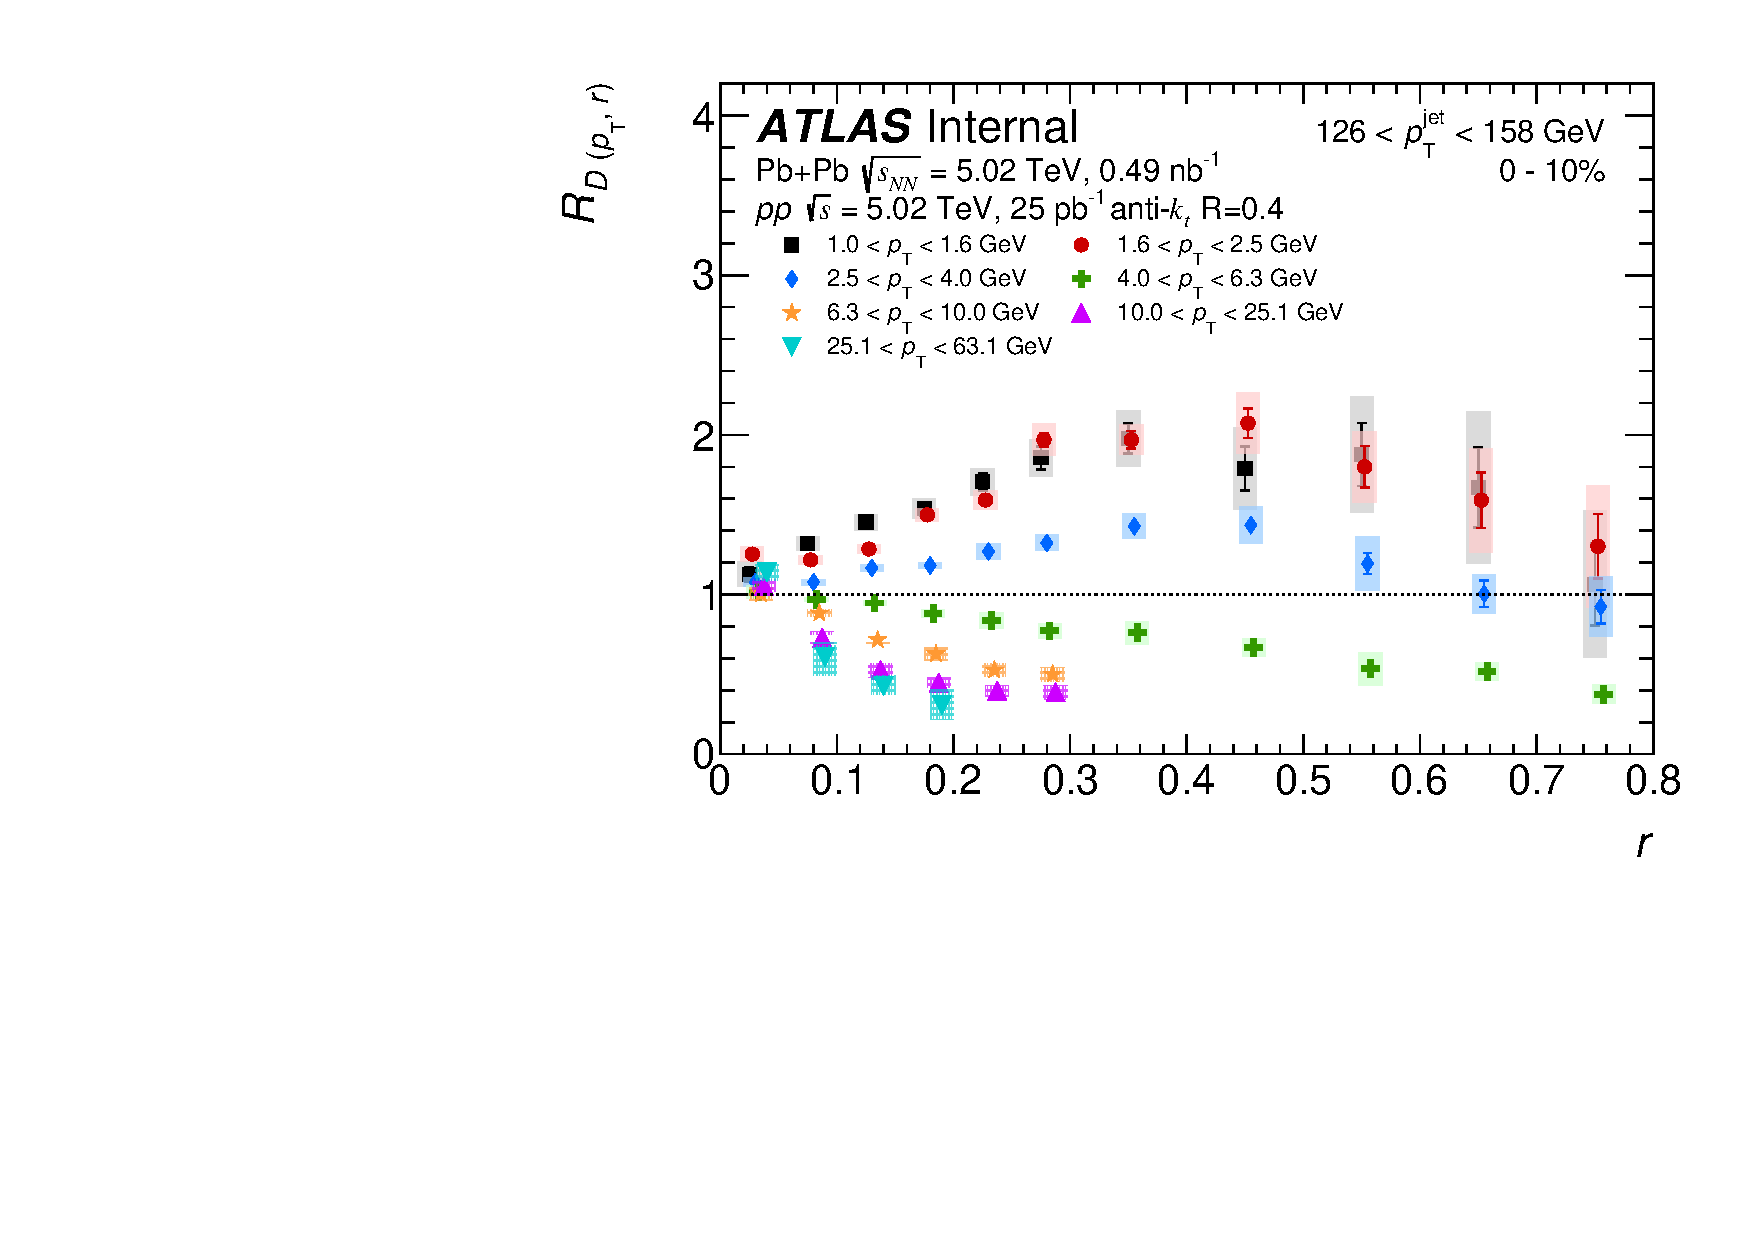
\includegraphics[width=0.5\textwidth]{figures/results/RDpT_dR_jet7_cent0.pdf} & 
            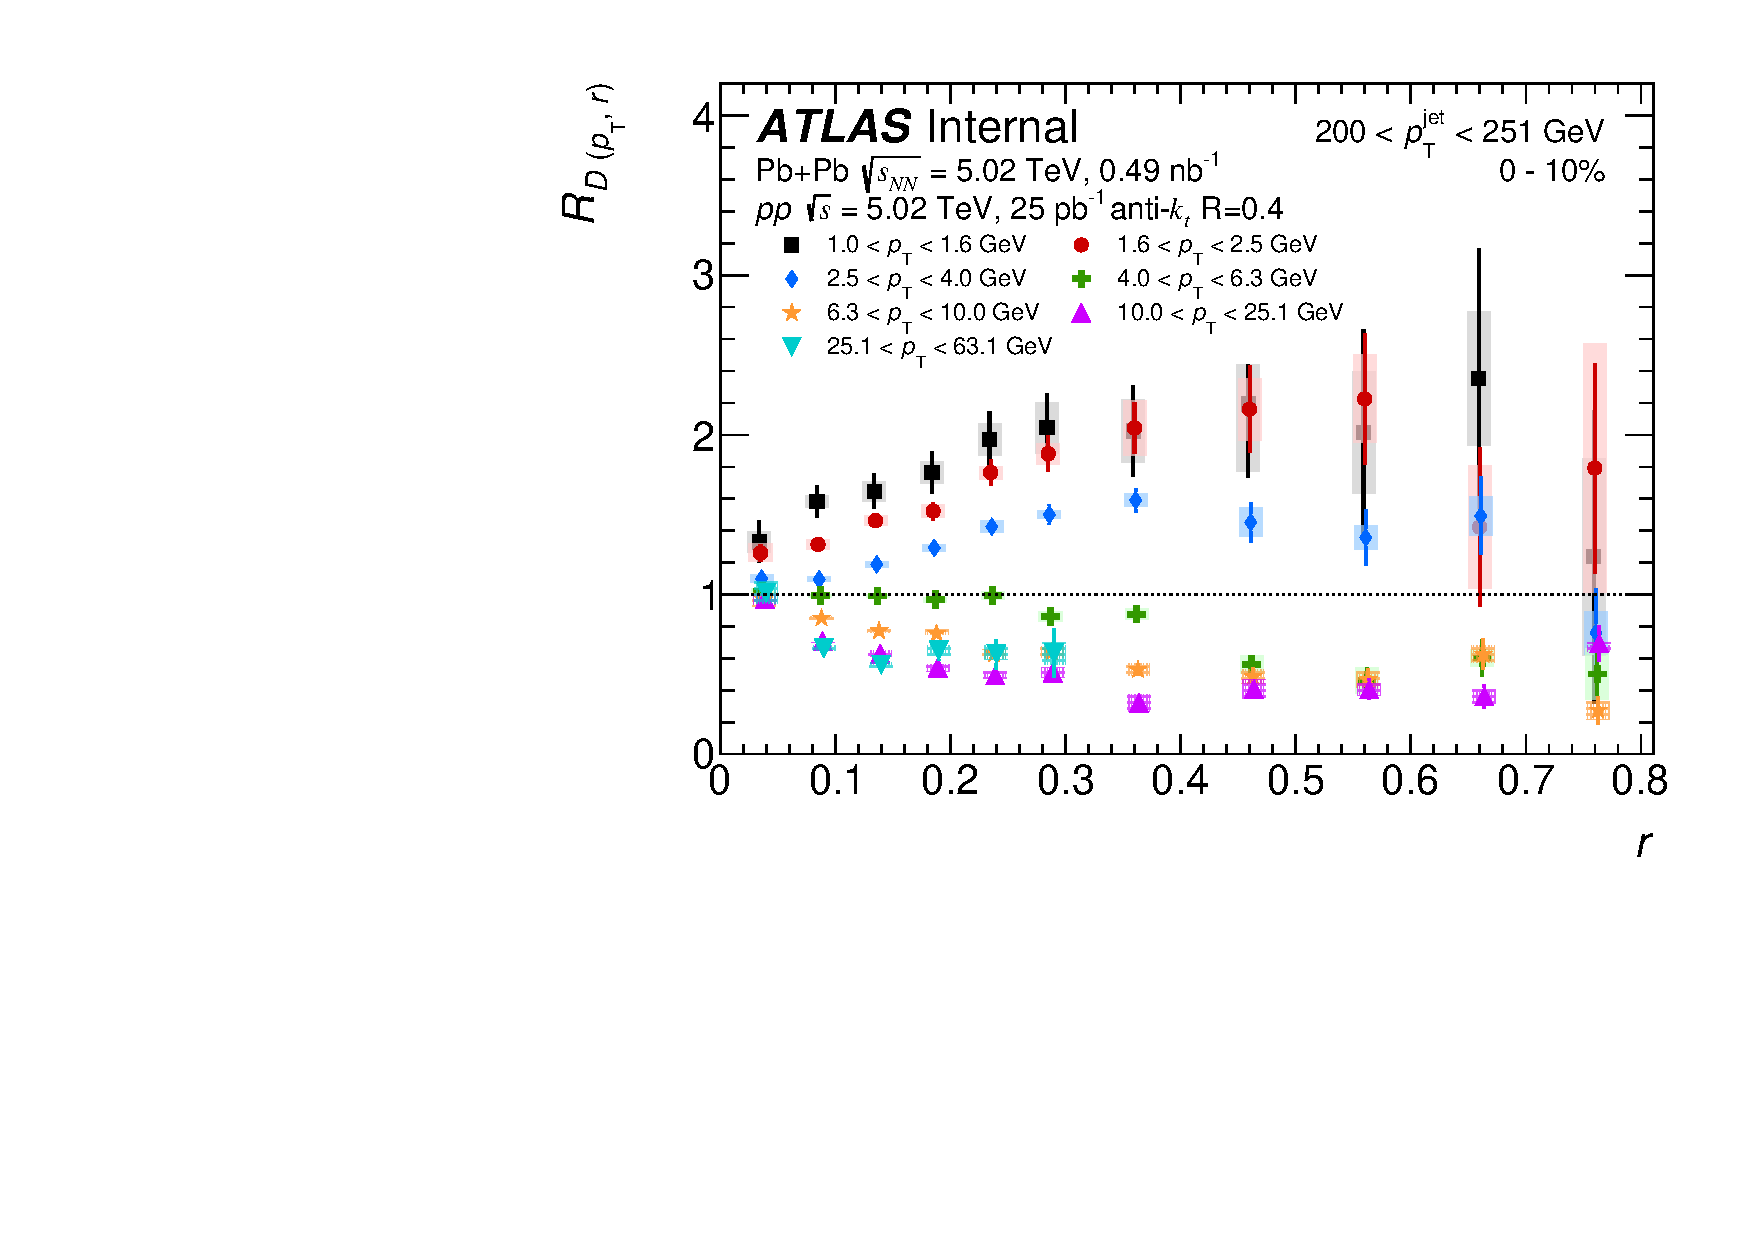
\includegraphics[width=0.5\textwidth]{figures/results/RDpT_dR_jet9_cent0.pdf} \\
            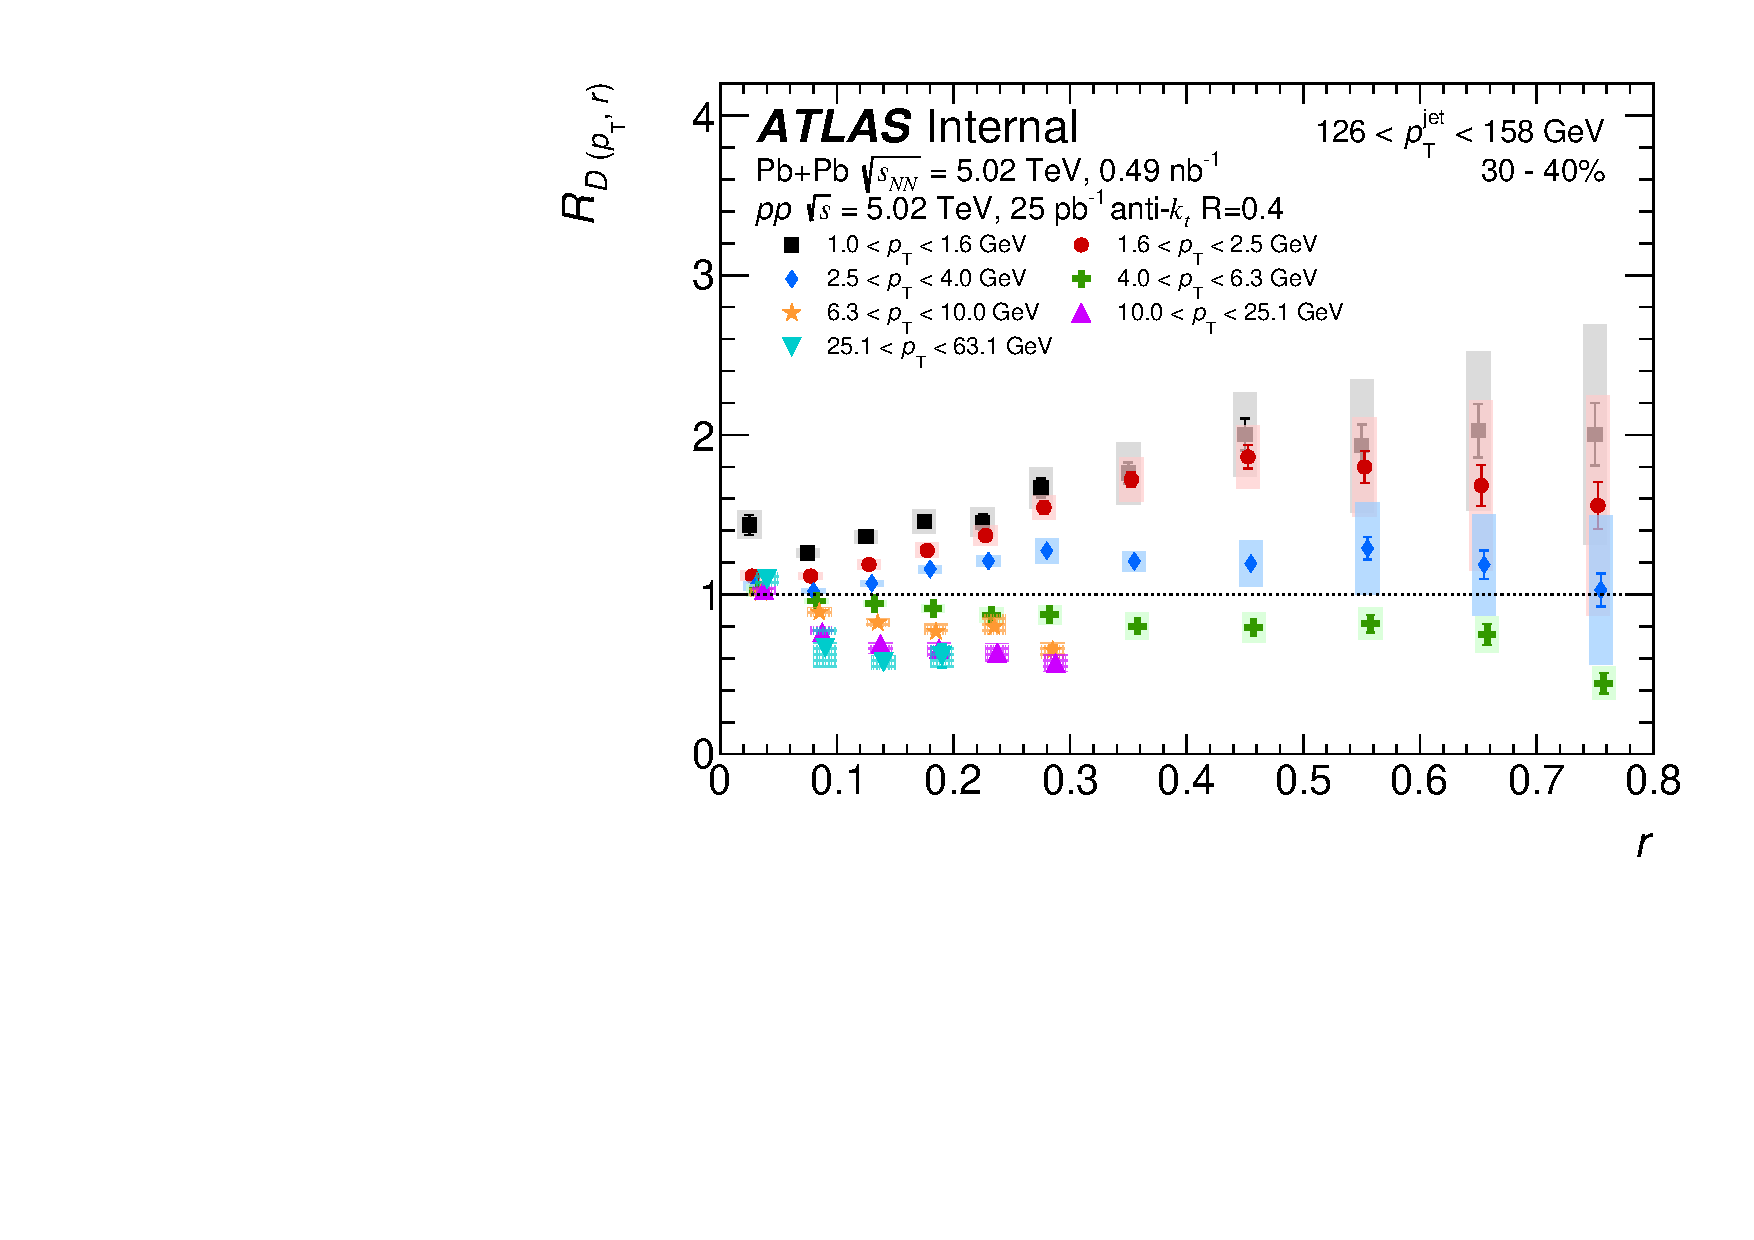
\includegraphics[width=0.5\textwidth]{figures/results/RDpT_dR_jet7_cent3.pdf} & 
            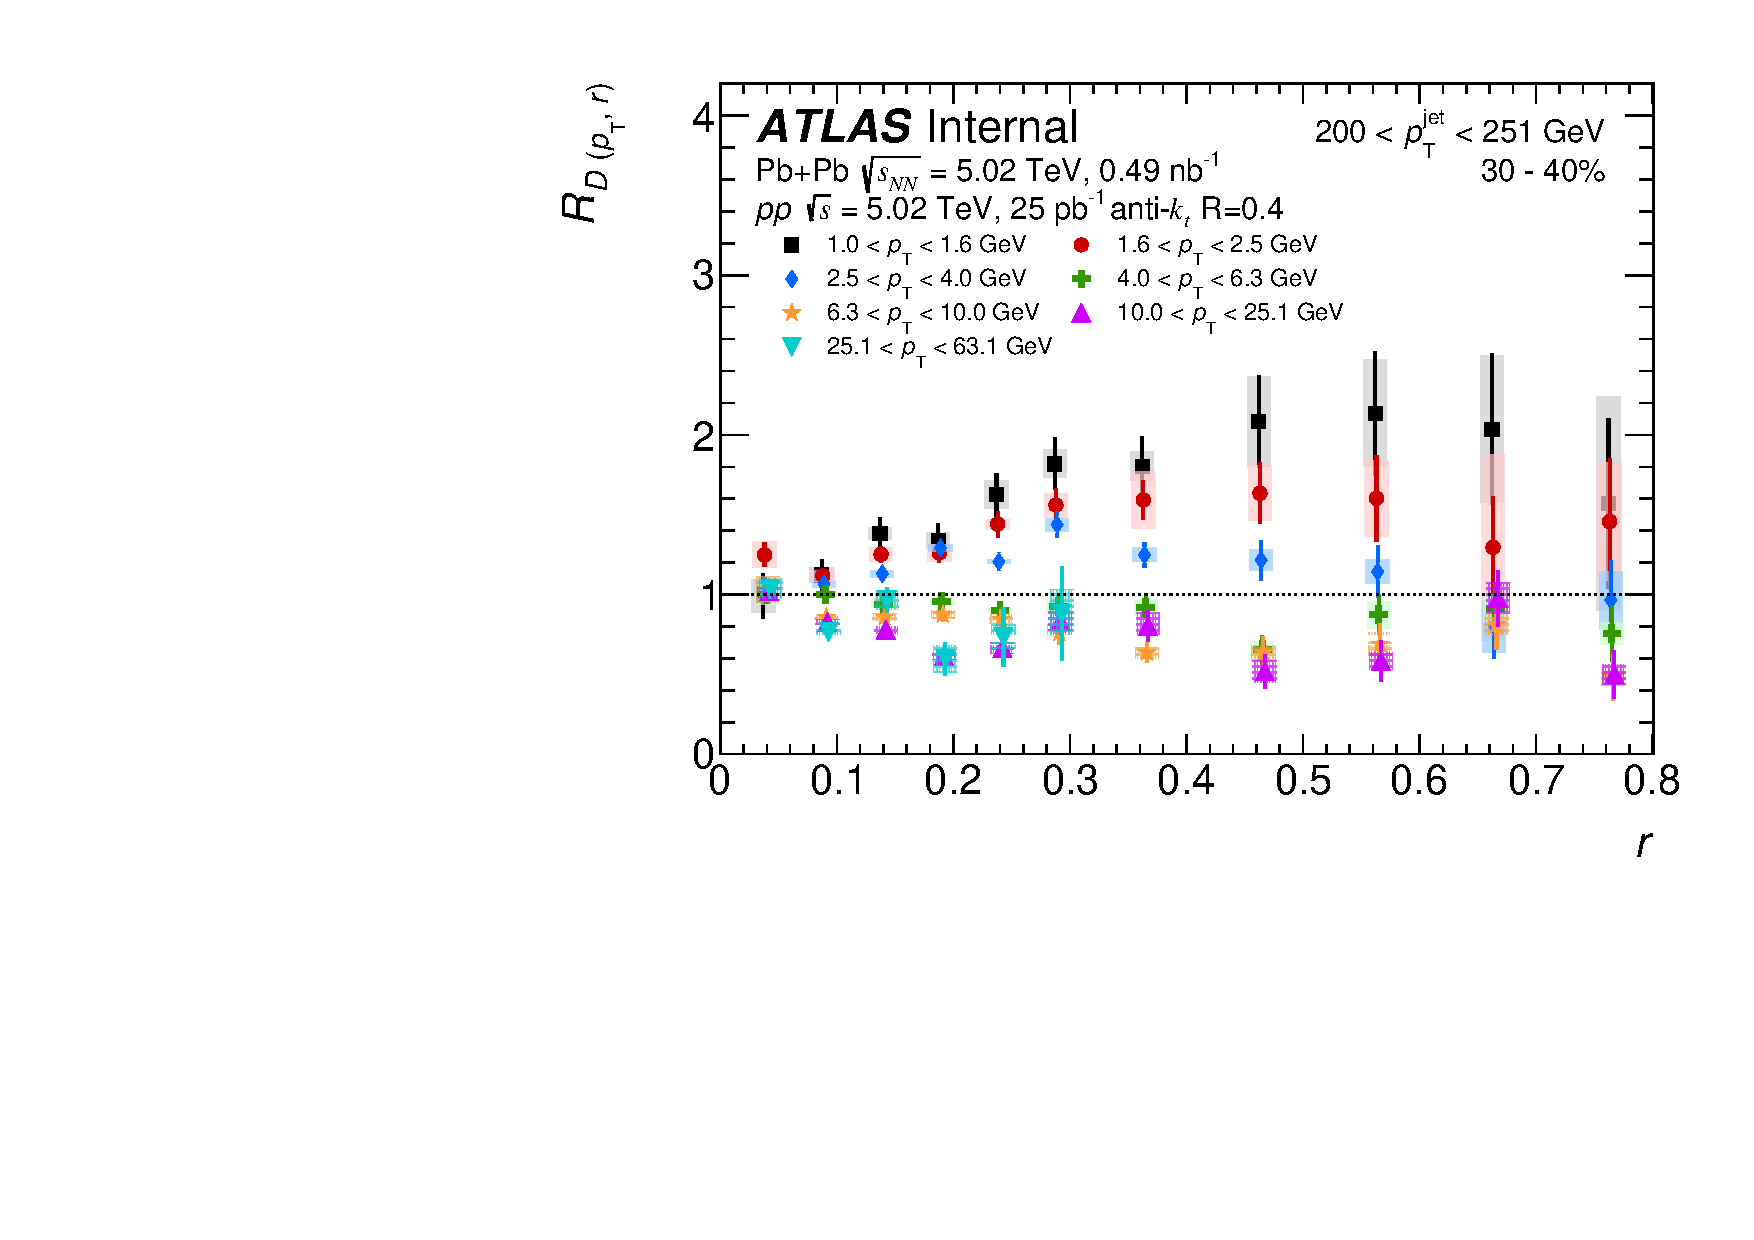
\includegraphics[width=0.5\textwidth]{figures/results/RDpT_dR_jet9_cent3.pdf} \\
            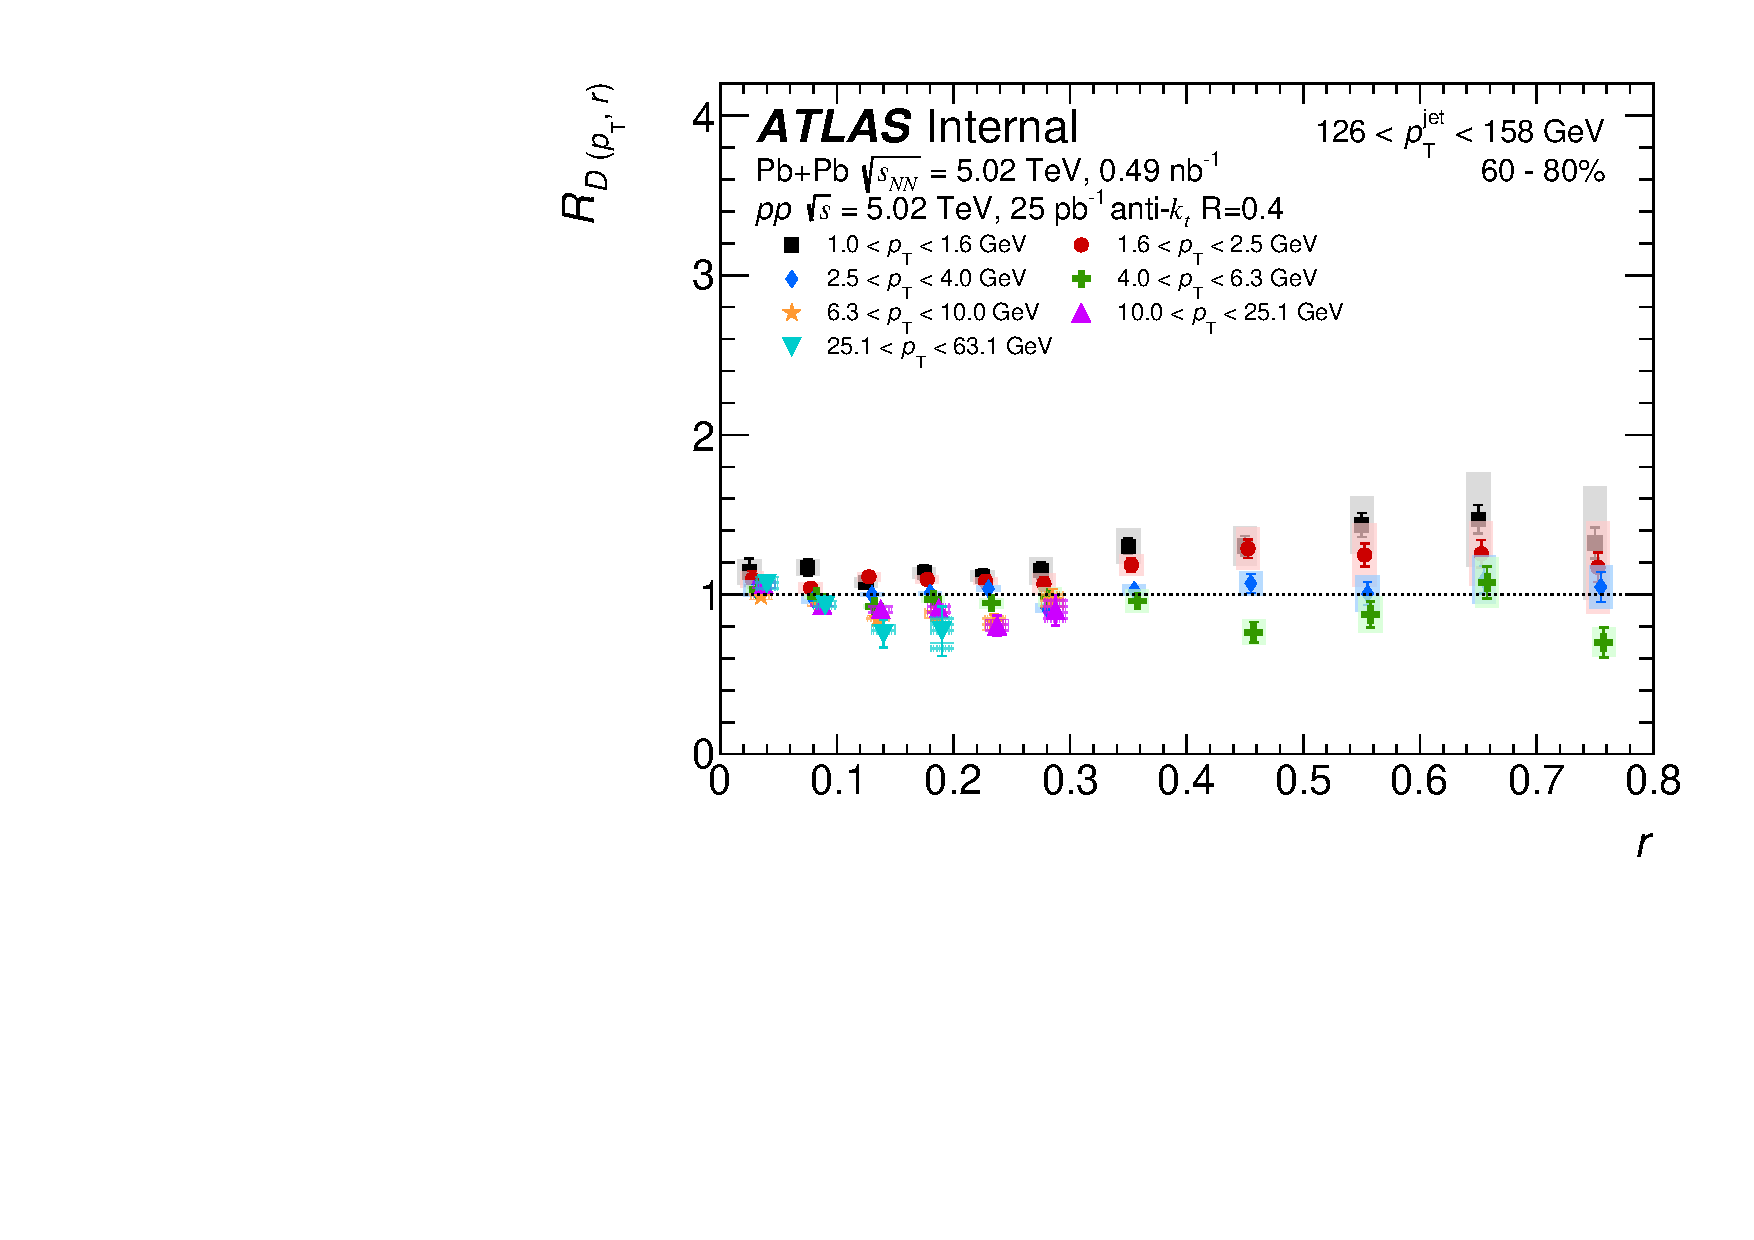
\includegraphics[width=0.5\textwidth]{figures/results/RDpT_dR_jet7_cent5.pdf} & 
            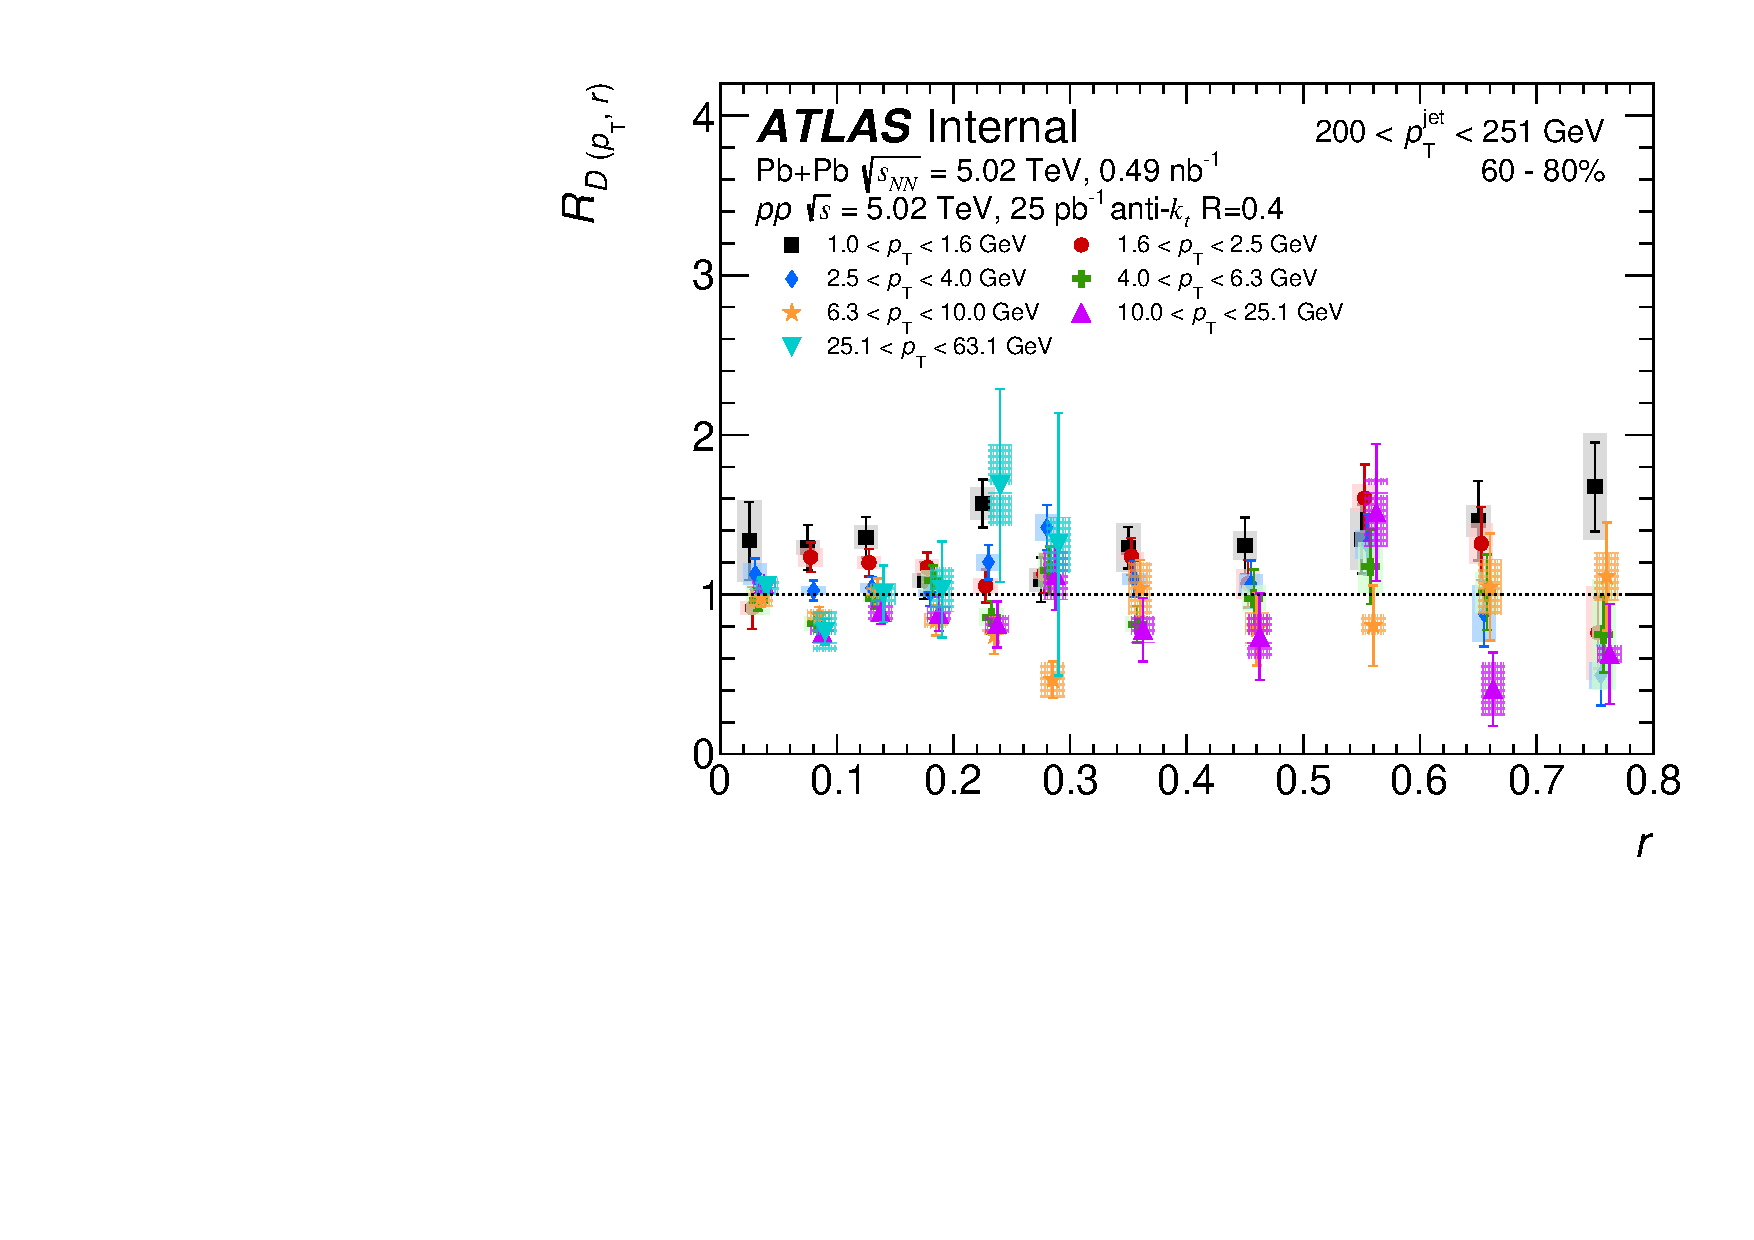
\includegraphics[width=0.5\textwidth]{figures/results/RDpT_dR_jet9_cent5.pdf} \\
      \end{tabular}
      }
\caption{Ratios of \Dptr\ distributions in 0--10\% (top), 30--40\% (middle), and 60--80\% (bottom) \PbPb\ collisions to \pp\ collisions as a function of angular distance $r$ for \ptjet\ of 126 to 158~\GeV\ (left) and of 200 to 251~\GeV\ (right) for six \pt\ selections. The vertical bars on the data points indicate statistical uncertainties while the shaded boxes indicate systematic uncertainties. The widths of the boxes are not indicative of the bin size and the points are shifted horizontally for better visibility.}
\label{fig:rdptr}
\end{figure}


% This observation is in agreement with the previous measurement of jet fragmentation functions \cite{Chatrchyan:2014ava, Sirunyan:2018jqr, Aaboud:2017bzv, PhysRevC.98.024908} and may indicate the dependence of the response of the hot dense matter to the momentum of a jet passing through it. 


\FloatBarrier
